\documentclass[11pt,a4paper,]{article}
\usepackage{lmodern}

\usepackage{amssymb,amsmath}
\usepackage{ifxetex,ifluatex}
\usepackage{fixltx2e} % provides \textsubscript
\ifnum 0\ifxetex 1\fi\ifluatex 1\fi=0 % if pdftex
  \usepackage[T1]{fontenc}
  \usepackage[utf8]{inputenc}
\else % if luatex or xelatex
  \usepackage{unicode-math}
  \defaultfontfeatures{Ligatures=TeX,Scale=MatchLowercase}
\fi
% use upquote if available, for straight quotes in verbatim environments
\IfFileExists{upquote.sty}{\usepackage{upquote}}{}
% use microtype if available
\IfFileExists{microtype.sty}{%
\usepackage[]{microtype}
\UseMicrotypeSet[protrusion]{basicmath} % disable protrusion for tt fonts
}{}
\PassOptionsToPackage{hyphens}{url} % url is loaded by hyperref
\usepackage[unicode=true]{hyperref}
\hypersetup{
            pdftitle={CO2 Emission Analysis},
            pdfborder={0 0 0},
            breaklinks=true}
\urlstyle{same}  % don't use monospace font for urls
\usepackage{geometry}
\geometry{a4paper, centering, text={16cm,24cm}}
\usepackage[style=authoryear-comp,]{biblatex}
\addbibresource{references.bib}
\usepackage{longtable,booktabs}
% Fix footnotes in tables (requires footnote package)
\IfFileExists{footnote.sty}{\usepackage{footnote}\makesavenoteenv{long table}}{}
\IfFileExists{parskip.sty}{%
\usepackage{parskip}
}{% else
\setlength{\parindent}{0pt}
\setlength{\parskip}{6pt plus 2pt minus 1pt}
}
\setlength{\emergencystretch}{3em}  % prevent overfull lines
\providecommand{\tightlist}{%
  \setlength{\itemsep}{0pt}\setlength{\parskip}{0pt}}
\setcounter{secnumdepth}{5}

% set default figure placement to htbp
\makeatletter
\def\fps@figure{htbp}
\makeatother


\title{CO2 Emission Analysis}

%% MONASH STUFF

%% CAPTIONS
\RequirePackage{caption}
\DeclareCaptionStyle{italic}[justification=centering]
 {labelfont={bf},textfont={it},labelsep=colon}
\captionsetup[figure]{style=italic,format=hang,singlelinecheck=true}
\captionsetup[table]{style=italic,format=hang,singlelinecheck=true}


%% FONT
\RequirePackage{bera}
\RequirePackage[charter,expert,sfscaled]{mathdesign}
\RequirePackage{fontawesome}

%% HEADERS AND FOOTERS
\RequirePackage{fancyhdr}
\pagestyle{fancy}
\rfoot{\Large\sffamily\raisebox{-0.1cm}{\textbf{\thepage}}}
\makeatletter
\lhead{\textsf{\expandafter{\@title}}}
\makeatother
\rhead{}
\cfoot{}
\setlength{\headheight}{15pt}
\renewcommand{\headrulewidth}{0.4pt}
\renewcommand{\footrulewidth}{0.4pt}
\fancypagestyle{plain}{%
\fancyhf{} % clear all header and footer fields
\fancyfoot[C]{\sffamily\thepage} % except the center
\renewcommand{\headrulewidth}{0pt}
\renewcommand{\footrulewidth}{0pt}}

%% MATHS
\RequirePackage{bm,amsmath}
\allowdisplaybreaks

%% GRAPHICS
\RequirePackage{graphicx}
\setcounter{topnumber}{2}
\setcounter{bottomnumber}{2}
\setcounter{totalnumber}{4}
\renewcommand{\topfraction}{0.85}
\renewcommand{\bottomfraction}{0.85}
\renewcommand{\textfraction}{0.15}
\renewcommand{\floatpagefraction}{0.8}


%\RequirePackage[section]{placeins}

%% SECTION TITLES


%% SECTION TITLES (NEW: Changing sections and subsections color)
\RequirePackage[compact,sf,bf]{titlesec}
\titleformat*{\section}{\Large\sf\bfseries\color[rgb]{0.8, 0.7, 0.1 }}
\titleformat*{\subsection}{\large\sf\bfseries\color[rgb]{0.8, 0.7, 0.1 }}
\titleformat*{\subsubsection}{\sf\bfseries\color[rgb]{0.8, 0.7, 0.1 }}
\titlespacing{\section}{0pt}{2ex}{.5ex}
\titlespacing{\subsection}{0pt}{1.5ex}{0ex}
\titlespacing{\subsubsection}{0pt}{.5ex}{0ex}


%% TITLE PAGE
\def\Date{\number\day}
\def\Month{\ifcase\month\or
 January\or February\or March\or April\or May\or June\or
 July\or August\or September\or October\or November\or December\fi}
\def\Year{\number\year}

%% LINE AND PAGE BREAKING
\sloppy
\clubpenalty = 10000
\widowpenalty = 10000
\brokenpenalty = 10000
\RequirePackage{microtype}

%% PARAGRAPH BREAKS
\setlength{\parskip}{1.4ex}
\setlength{\parindent}{0em}

%% HYPERLINKS
\RequirePackage{xcolor} % Needed for links
\definecolor{darkblue}{rgb}{0,0,.6}
\RequirePackage{url}

\makeatletter
\@ifpackageloaded{hyperref}{}{\RequirePackage{hyperref}}
\makeatother
\hypersetup{
     citecolor=0 0 0,
     breaklinks=true,
     bookmarksopen=true,
     bookmarksnumbered=true,
     linkcolor=darkblue,
     urlcolor=blue,
     citecolor=darkblue,
     colorlinks=true}

\usepackage[showonlyrefs]{mathtools}
\usepackage[no-weekday]{eukdate}

%% BIBLIOGRAPHY

\makeatletter
\@ifpackageloaded{biblatex}{}{\usepackage[style=authoryear-comp, backend=biber, natbib=true]{biblatex}}
\makeatother
\ExecuteBibliographyOptions{bibencoding=utf8,minnames=1,maxnames=3, maxbibnames=99,dashed=false,terseinits=true,giveninits=true,uniquename=false,uniquelist=false,doi=false, isbn=false,url=true,sortcites=false}

\DeclareFieldFormat{url}{\texttt{\url{#1}}}
\DeclareFieldFormat[article]{pages}{#1}
\DeclareFieldFormat[inproceedings]{pages}{\lowercase{pp.}#1}
\DeclareFieldFormat[incollection]{pages}{\lowercase{pp.}#1}
\DeclareFieldFormat[article]{volume}{\mkbibbold{#1}}
\DeclareFieldFormat[article]{number}{\mkbibparens{#1}}
\DeclareFieldFormat[article]{title}{\MakeCapital{#1}}
\DeclareFieldFormat[article]{url}{}
%\DeclareFieldFormat[book]{url}{}
%\DeclareFieldFormat[inbook]{url}{}
%\DeclareFieldFormat[incollection]{url}{}
%\DeclareFieldFormat[inproceedings]{url}{}
\DeclareFieldFormat[inproceedings]{title}{#1}
\DeclareFieldFormat{shorthandwidth}{#1}
%\DeclareFieldFormat{extrayear}{}
% No dot before number of articles
\usepackage{xpatch}
\xpatchbibmacro{volume+number+eid}{\setunit*{\adddot}}{}{}{}
% Remove In: for an article.
\renewbibmacro{in:}{%
  \ifentrytype{article}{}{%
  \printtext{\bibstring{in}\intitlepunct}}}

\AtEveryBibitem{\clearfield{month}}
\AtEveryCitekey{\clearfield{month}}

\makeatletter
\DeclareDelimFormat[cbx@textcite]{nameyeardelim}{\addspace}
\makeatother

\author{\sf\Large\textbf{ Ziyao Wang}\\ {\sf\large MBAt\\[0.5cm]} \sf\Large\textbf{ Jiaying Zhang}\\ {\sf\large MBAt\\[0.5cm]} \sf\Large\textbf{ Karan Garg}\\ {\sf\large MBAt\\[0.5cm]}}

\date{\sf\Date~\Month~\Year}
\makeatletter
\lfoot{\sf Wang, Zhang, Garg: \@date}
\makeatother


%%%% PAGE STYLE FOR FRONT PAGE OF REPORTS

\makeatletter
\def\organization#1{\gdef\@organization{#1}}
\def\telephone#1{\gdef\@telephone{#1}}
\def\email#1{\gdef\@email{#1}}
\makeatother
  \organization{Monash University,Clayton}

  \def\name{Our consultancy \newline Department of Econometrics and Business Statistics \newline Monash business school}

  \telephone{(03) 9905 2478}

  \email{questions@company.com}                 %NEW: New email addresss

\def\webaddress{\url{http://company.com/stats/consulting/}} %NEW: URl
\def\abn{12 377 614 630}                                    % NEW: ABN
\def\logo{\includegraphics[width=6cm]{Figures/logo}}  %NEW: Changing logo
\def\extraspace{\vspace*{1.6cm}}
\makeatletter
\def\contactdetails{\faicon{phone} & \@telephone \\
                    \faicon{envelope} & \@email}
\makeatother

%%%% FRONT PAGE OF REPORTS

\def\reporttype{Report for}

\long\def\front#1#2#3{
\newpage
\begin{singlespacing}
\thispagestyle{empty}
\vspace*{-1.4cm}
\hspace*{-1.4cm}
\hbox to 16cm{
  \hbox to 6.5cm{\vbox to 14cm{\vbox to 25cm{
    \logo
    \vfill
    \parbox{6.3cm}{\raggedright
      \sf\color[rgb]{0.8, 0.7, 0.1 }    % NEW color 
      {\large\textbf{\name}}\par
      \vspace{.7cm}
      \tabcolsep=0.12cm\sf\small
      \begin{tabular}{@{}ll@{}}\contactdetails
      \end{tabular}
      \vspace*{0.3cm}\par
      ABN: \abn\par
    }
  }\vss}\hss}
  \hspace*{0.2cm}
  \hbox to 1cm{\vbox to 14cm{\rule{4pt}{26.8cm}\vss}\hss\hfill}  %NEW: Thicker line
  \hbox to 10cm{\vbox to 14cm{\vbox to 25cm{   
      \vspace*{3cm}\sf\raggedright
      \parbox{11cm}{\sf\raggedright\baselineskip=1.2cm
         \fontsize{24.88}{30}\color[rgb]{0, 0.29, 0.55}\sf\textbf{#1}}   % NEW: title color blue
      \par
      \vfill
      \large
      \vbox{\parskip=0.8cm #2}\par
      \vspace*{2cm}\par
      \reporttype\\[0.3cm]
      \hbox{#3}%\\[2cm]\
      \vspace*{1cm}
      {\large\sf\textbf{\Date~\Month~\Year}}
   }\vss}
  }}
\end{singlespacing}
\newpage
}

\makeatletter
\def\titlepage{\front{\expandafter{\@title}}{\@author}{\@organization}}
\makeatother

\usepackage{setspace}
\setstretch{1.5}

%% Any special functions or other packages can be loaded here.
\usepackage{booktabs}
\usepackage{longtable}
\usepackage{array}
\usepackage{multirow}
\usepackage{wrapfig}
\usepackage{float}
\usepackage{colortbl}
\usepackage{pdflscape}
\usepackage{tabu}
\usepackage{threeparttable}
\usepackage{threeparttablex}
\usepackage[normalem]{ulem}
\usepackage{makecell}
\usepackage{xcolor}


\begin{document}
\titlepage

{
\setcounter{tocdepth}{2}
\tableofcontents
}
\clearpage

\hypertarget{section-1---country-chn-and-usa}{%
\section{Section 1 - Country CHN and USA}\label{section-1---country-chn-and-usa}}

\hypertarget{introduction---research-questions}{%
\subsection{Introduction - research questions}\label{introduction---research-questions}}

This section will focus on the CO2 emissions between China and the USA and try to discover any possible factors that are associated with the emissions.

Q1: How do China and the USA's CO2 emissions change over time?\\
Q2: Are CO2 emissions correlated with the urban population? Is the increase in population necessary will increase the CO2 emissions per capita?

\hypertarget{co2-emissions-change-over-time.}{%
\subsection{CO2 emissions change over time.}\label{co2-emissions-change-over-time.}}

The table \ref{tab:sumtable} suggests that the USA has a higher CO2 emission per capita than China's through observing the median values.

\begin{table}[!h]

\caption{\label{tab:sumtable}CO2 Emissions per capita summary}
\centering
\begin{tabular}[t]{rrrl}
\toprule
Min\_emission & Median\_emission & Max\_emission & Country\_Name\\
\midrule
\cellcolor{gray!6}{0.5741621} & \cellcolor{gray!6}{2.038411} & \cellcolor{gray!6}{7.557211} & \cellcolor{gray!6}{China}\\
15.6812555 & 19.347083 & 22.510582 & USA\\
\bottomrule
\end{tabular}
\end{table}

\clearpage

\begin{figure}

{\centering 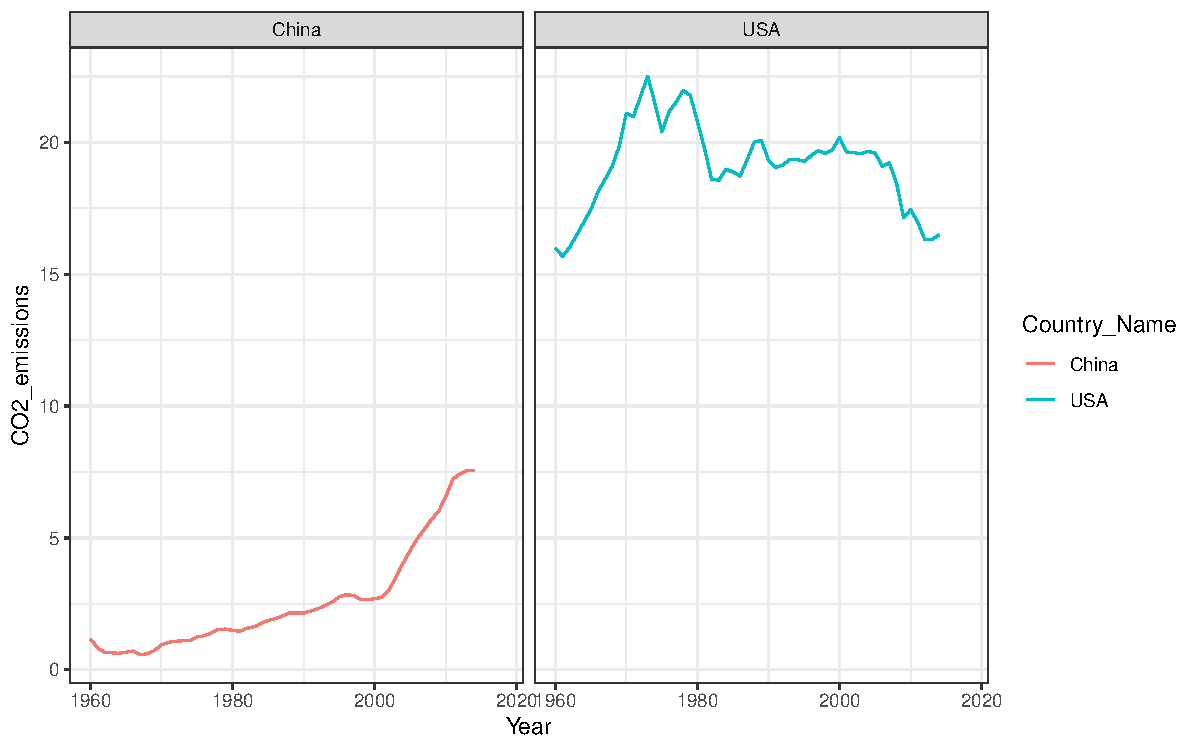
\includegraphics[width=0.5\linewidth]{Figures/figure1-1} 

}

\caption{CO2 Emissions per Capita over time}\label{fig:figure1}
\end{figure}

The line charts \ref{fig:figure1} present the CO2 emissions changes over time for each country. According to the report of \textcite{SUEWING20075267}, it states that since 2005 the USA is undergoing a shift in its energy generation mix from coal to natural gas, which leads to a significant reduction on the CO2 emission. Thus, the USA's CO2 emission per capita is in a decreasing trend.

\hypertarget{relationship-between-co2-emissions-and-urban-population.}{%
\subsection{Relationship between CO2 emissions and urban population.}\label{relationship-between-co2-emissions-and-urban-population.}}

\begin{figure}

{\centering 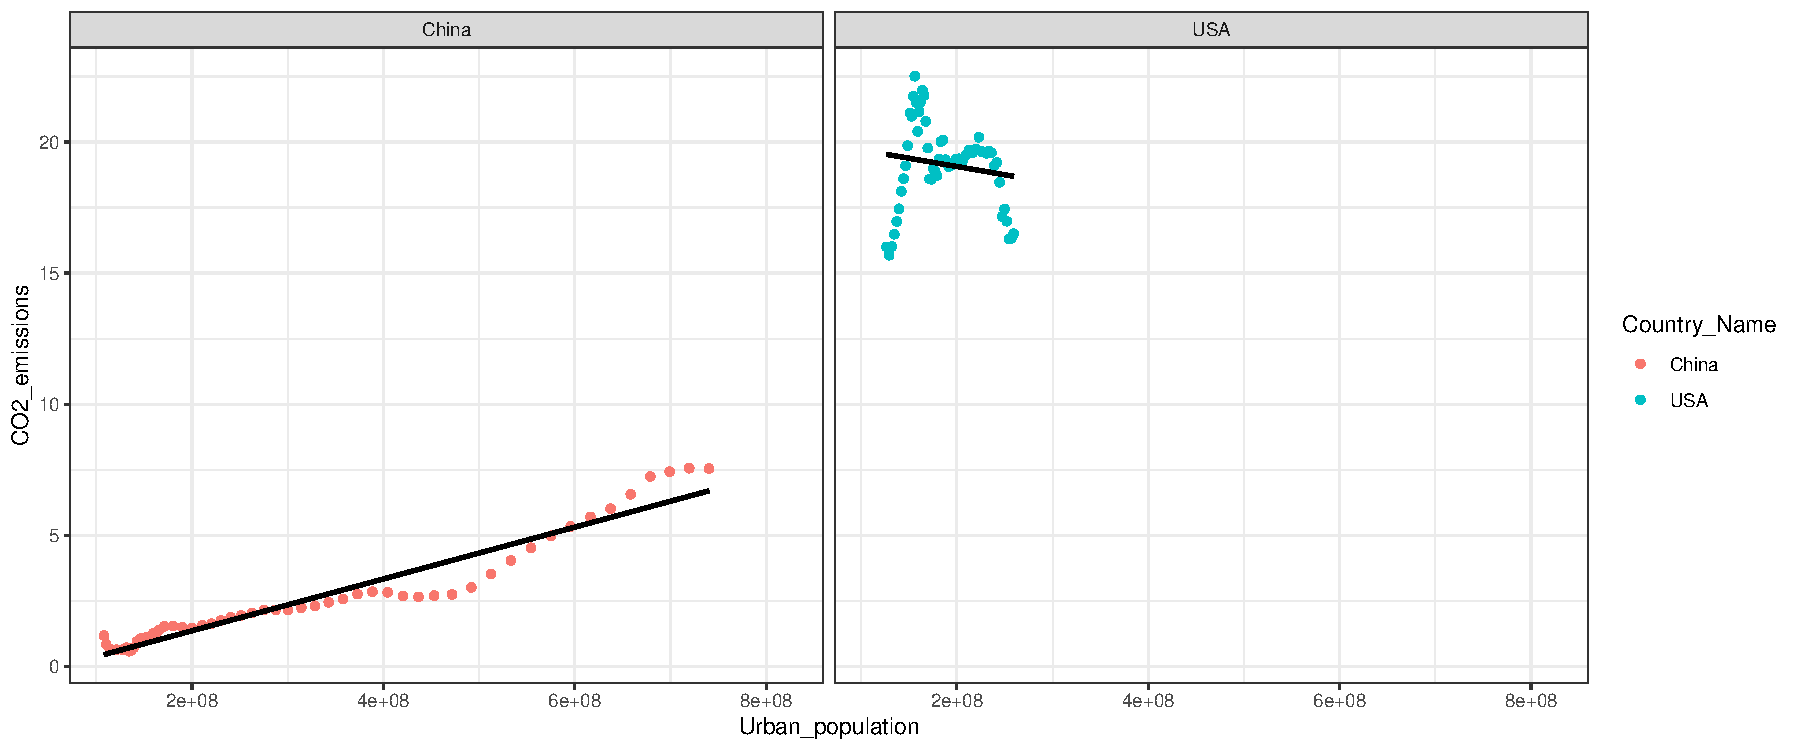
\includegraphics[width=0.8\linewidth]{Figures/scatterplot-1} 

}

\caption{Scatter plots for each country}\label{fig:scatterplot}
\end{figure}

The figures \ref{fig:scatterplot}, they suggest that the urban population may be a useful explanatory to CO2 emission for China yet not for the USA's. From the linear model, China one has an R squared of 0.9270993 and USA one is 0.0225544.

\clearpage

\hypertarget{section-2---country-iceland-and-thailand}{%
\section{Section 2 - Country Iceland and Thailand}\label{section-2---country-iceland-and-thailand}}

\textbf{Introduction} :
This part focuses on CO2 emissions of Iceland and Thailand. It analyzes the change of CO2 emissions, average annual increase of CO2 emissions during 45 years and explores the relationship between CO2 emissions per person and energy use per person in these two countries.

\hypertarget{how-did-the-co2-emissions-of-iceland-and-thailand-change-from-1971-to-2014-and-how-much-did-they-change-on-average-each-year}{%
\subsection{How did the CO2 emissions of Iceland and Thailand change from 1971 to 2014, and how much did they change on average each year?}\label{how-did-the-co2-emissions-of-iceland-and-thailand-change-from-1971-to-2014-and-how-much-did-they-change-on-average-each-year}}

\begin{table}[!h]

\caption{\label{tab:co2table}The summary of CO2 emissions of Iceland and Thailand}
\centering
\begin{tabular}[t]{lrrrrr}
\toprule
Country\_Name & average & min & max & range & change\_per\_year\\
\midrule
\cellcolor{gray!6}{Iceland} & \cellcolor{gray!6}{7.34} & \cellcolor{gray!6}{5.61} & \cellcolor{gray!6}{8.80} & \cellcolor{gray!6}{3.19} & \cellcolor{gray!6}{0.07}\\
Thailand & 2.20 & 0.51 & 4.62 & 4.11 & 0.09\\
\bottomrule
\end{tabular}
\end{table}

As shown in Table \ref{tab:co2table},we can see the summary of the situation of CO2 emission in Thailand and Iceland. From 2015 to 2018, \textbf{Iceland}'s average CO2 emission was Thailand was much \textbf{higher} than that of \textbf{7.34} (2.2), but \textbf{Thailand}'s growth rate was \textbf{faster} 0.09 per year, while Iceland's was 0.07 per year.

\hypertarget{are-co2-emissions-per-person-related-to-energy-use-per-person-what-is-the-connection-between-them}{%
\subsection{Are CO2 emissions per person related to energy use per person? What is the connection between them?}\label{are-co2-emissions-per-person-related-to-energy-use-per-person-what-is-the-connection-between-them}}

\begin{figure}

{\centering 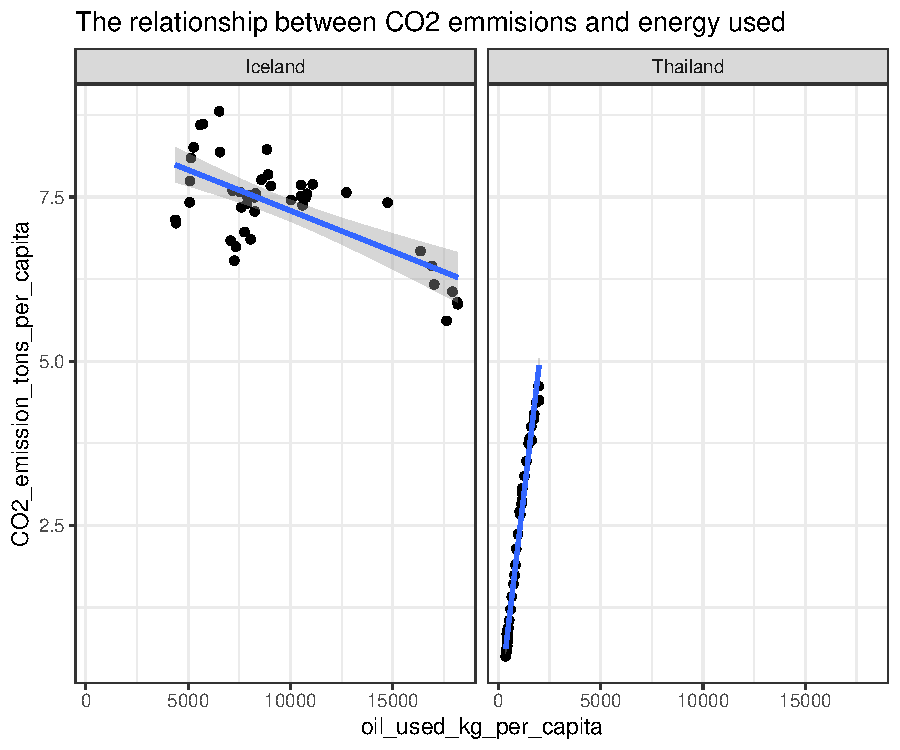
\includegraphics{Figures/relationship-1} 

}

\caption{The relationship between CO2 emissions and energy used}\label{fig:relationship}
\end{figure}

The relationship between CO2 emissions and energy use are displayed in \ref{fig:relationship}.
\clearpage
In Thailand and Iceland, the relationships between CO2 emissions and energy use are very \textbf{different}. I used linear model to make the relation between these two attributes became more obviously. In \textbf{Thailand}, there is an obvious \textbf{positive correlation} between \textbf{carbon dioxide emissions} and the amount of \textbf{oil used}, while in \textbf{Iceland}, although not as obvious as in Thailand, it shows a \textbf{negative correlation}.

Carbon dioxide and oil use in Iceland have been \textbf{growing slowly} or even falling in recent years. Refer to the report \textcite{CookDavid2016EpiI}, this phenomenon may related to the rapid development of Iceland's renewable energy industry in recent years, with its abundant hydropower and geothermal sources together now supplying almost 100\% of electricity generation and 85\% of primary energy use, which \textbf{decrease} the emission of CO2.

\textbf{Conclusion}:
1) Thailand's per capita carbon dioxide emissions are not as high as Iceland's, but growing faster in recent years.
2) Carbon dioxide emissions and fuel consumption were significantly positively correlated in Thailand and negatively correlated in Iceland.

\clearpage

\hypertarget{section-3---country-india-and-uk}{%
\section{Section 3 - Country India and UK}\label{section-3---country-india-and-uk}}

This section showcases:

\begin{itemize}
\tightlist
\item
  How did CO@ emission ad Energy use varied in recent years depending upon population?
\item
  How did the CO2 emission varied over the years for both nations?
\item
  how did the population varied over the years for both nations?
\item
  Was there any relationship between CO2 emission and population?
\end{itemize}

I used packages \textcite{ggplot2} for graphical analysis

\hypertarget{tabular-analysis}{%
\subsection{Tabular analysis}\label{tabular-analysis}}

\begin{table}[!h]

\caption{\label{tab:statsis}CO2 Emission and Energy Use of India and UK when poulation was at its peak}
\centering
\begin{tabular}[t]{l|r|r|r|r}
\hline
Country & Year & CO2\_emission & Urban\_population & Energy\_use\\
\hline
\cellcolor{gray!6}{India} & \cellcolor{gray!6}{2018} & \cellcolor{gray!6}{1.253695} & \cellcolor{gray!6}{460295677} & \cellcolor{gray!6}{503.1283}\\
\hline
India & 2017 & 1.253695 & 449789369 & 503.1283\\
\hline
\cellcolor{gray!6}{India} & \cellcolor{gray!6}{2016} & \cellcolor{gray!6}{1.253695} & \cellcolor{gray!6}{439498772} & \cellcolor{gray!6}{503.1283}\\
\hline
India & 2015 & 1.253695 & 429428653 & 503.1283\\
\hline
\cellcolor{gray!6}{India} & \cellcolor{gray!6}{2014} & \cellcolor{gray!6}{1.727671} & \cellcolor{gray!6}{419568459} & \cellcolor{gray!6}{636.5702}\\
\hline
UK & 2018 & 8.254229 & 55450489 & 3355.6977\\
\hline
\cellcolor{gray!6}{UK} & \cellcolor{gray!6}{2017} & \cellcolor{gray!6}{8.254229} & \cellcolor{gray!6}{54923317} & \cellcolor{gray!6}{3355.6977}\\
\hline
UK & 2016 & 8.254229 & 54369540 & 3355.6977\\
\hline
\cellcolor{gray!6}{UK} & \cellcolor{gray!6}{2015} & \cellcolor{gray!6}{8.254229} & \cellcolor{gray!6}{53813373} & \cellcolor{gray!6}{2763.9801}\\
\hline
UK & 2014 & 6.497440 & 53218629 & 2776.8441\\
\hline
\end{tabular}
\end{table}

The table \ref{tab:statsis}, tells us that in recent years,With the increase n population:

\begin{itemize}
\tightlist
\item
  CO2 emission in \textbf{\emph{India}} slightly increased whereas for \textbf{\emph{UK}} it decreased.
\item
  Similarly, Energy use in \textbf{\emph{India}} decreased whereas for \textbf{\emph{UK}} it increased.
\end{itemize}

\clearpage

\hypertarget{graphical-analysis}{%
\subsection{Graphical Analysis}\label{graphical-analysis}}

\begin{figure}

{\centering 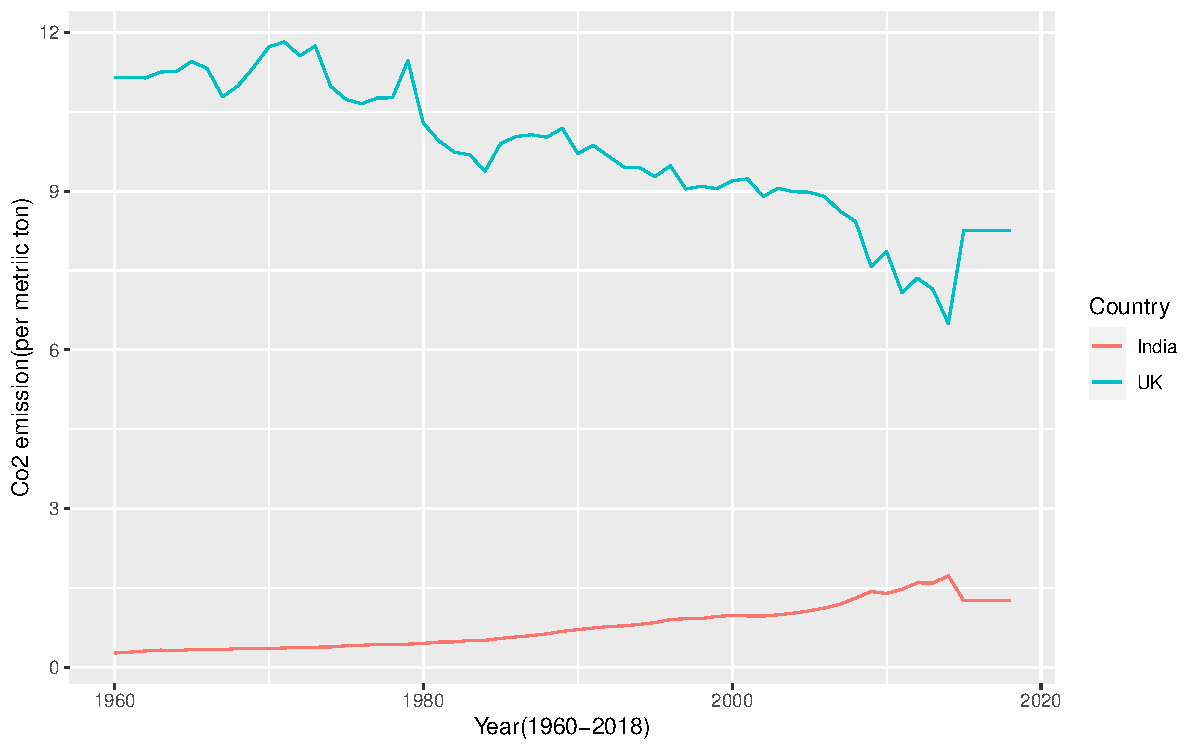
\includegraphics[width=0.9\linewidth]{Figures/co2-plt-1} 

}

\caption{Co2 Emission in India and UK from 1960 to 2018}\label{fig:co2-plt}
\end{figure}

The figure \ref{fig:co2-plt} tells us that:

\begin{itemize}
\tightlist
\item
  Overall CO2 emission was always more of \textbf{\emph{UK}} than \textbf{\emph{India}}.
\item
  CO2 emission was frequently changing in \textbf{\emph{UK}} and all in all was dropping to a min value of \textbf{6.5} in \textbf{2014} and then exponentially increased to \textbf{8.25}.
\item
  On other hand, in \textbf{\emph{India}} it remained pretty much stable and then started gradually increasing from \textbf{1984}.
\end{itemize}

\clearpage 
\begin{figure}

{\centering 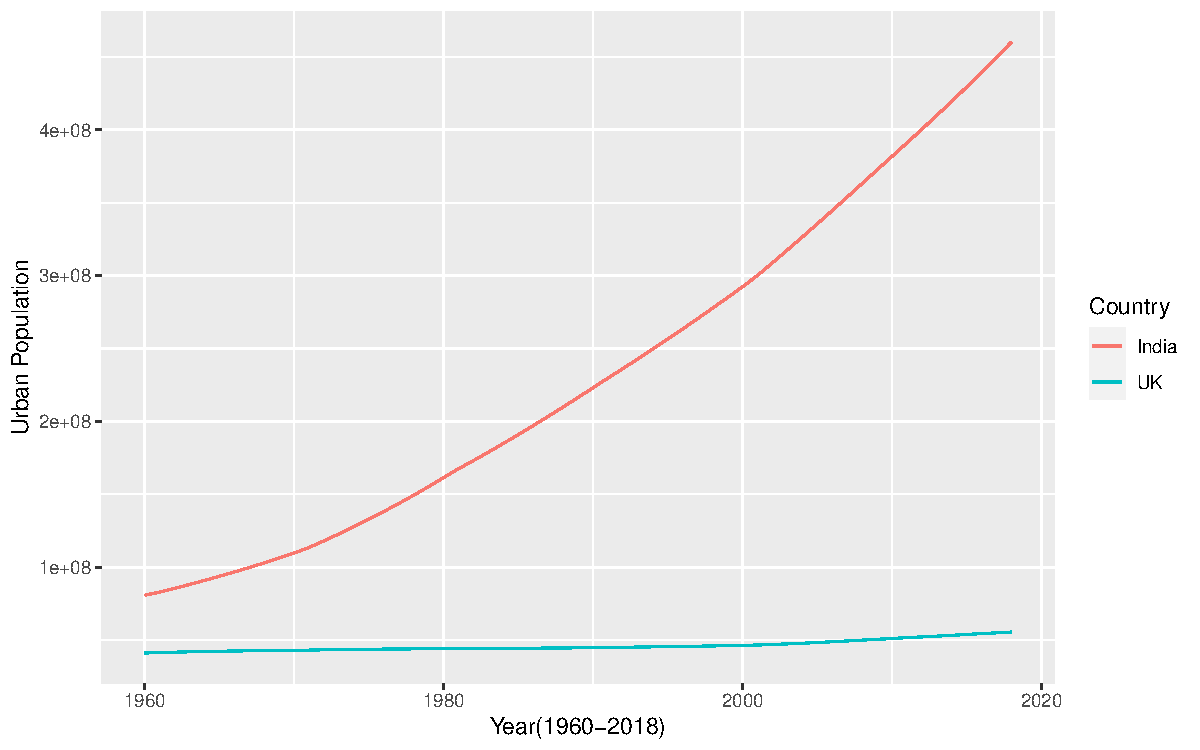
\includegraphics[width=0.9\linewidth]{Figures/popul-1} 

}

\caption{Population of UK and India from 1960-2018}\label{fig:popul}
\end{figure}

The figure \ref{fig:popul} tells us that population:

\begin{itemize}
\tightlist
\item
  In \textbf{\emph{India}} increased gradually but at the same time much faster than \textbf{\emph{UK}}.
\item
  In \textbf{\emph{UK}} it was pretty much the same in 20th Century, but had a slight increase in 21st Century.
\end{itemize}

\clearpage 
\begin{figure}

{\centering 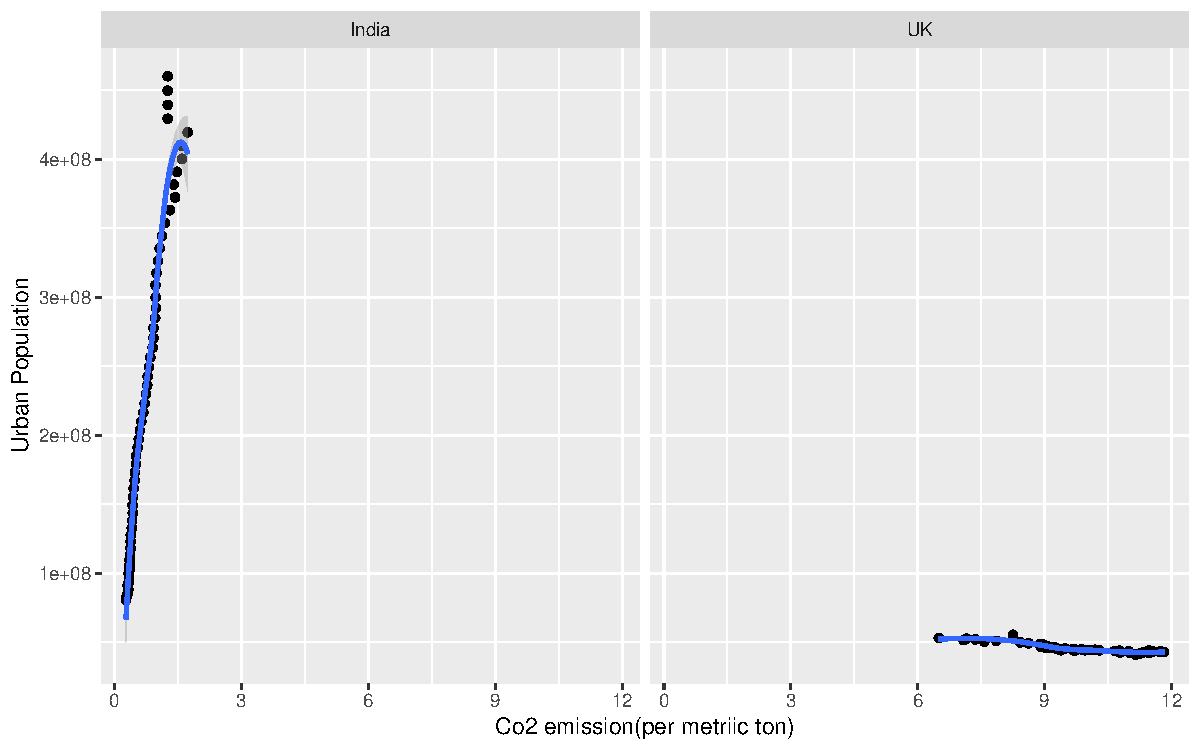
\includegraphics[width=0.9\linewidth]{Figures/rel-co2-pop-1} 

}

\caption{Relatioin between CO2 emission and Urban population}\label{fig:rel-co2-pop}
\end{figure}

The figure \ref{fig:rel-co2-pop} tells us that:

\begin{itemize}
\tightlist
\item
  Both for \textbf{\emph{India}} and \textbf{\emph{UK}}, increase in CO2 emission was related to Urban population and also tells us that the relation between the variables is strong(depicted by smooth line).
\end{itemize}

\hypertarget{conclusion-for-section-3}{%
\subsection{Conclusion for Section 3}\label{conclusion-for-section-3}}

\begin{itemize}
\tightlist
\item
  Increased CO2 emission in \textbf{\emph{UK}} is a surprising insight as the population is way less than \textbf{\emph{India}}.
\item
  On the other hand, Energy use is justified for both nations in respect to population.
\end{itemize}

\clearpage

\printbibliography

\end{document}
